
%%%%%%%%%%%%%%%%%%%%%
\chapter{Fonctions périodiques}
%%%%%%%%%%%%%%%%%%%%%

%%%%%%%%%%%%%%%%%%%%%
\section{Fonction périodique}
%%%%%%%%%%%%%%%%%%%%%
\subsection{Définition}
%%%%%%%%%%%%%%%%%%%%%
$\mc{F}_\mt{P}$(i) est une fonction périodique de période P, échantillonée (i est
entier). La période peut s'écrire comme la somme d'une puissance de deux ($2^\eta$)
et d'un nombre décimal $\rho$ inférieur à $2^\eta$ :
\[
\mt{P}=2^\eta+\rho\qquad\mt{avec}\qquad\rho<2^\eta
\]

$\mc{M}$(i) est un motif périodique de $\mc{F}_\mt{P}$(i). C'est une fonction de P
points. d est le déphasage de $\mc{F}_\mt{P}$ par rapport à $\mc{M}$.

La fonction périodique $\mc{F}_\mt{P}$(i) peut alors s'écrire :
\[
\mc{F}_\mt{P}\mt{(i)}=\mc{M}\big(\mt{ (i}+\mt{d) modulo P }\big)
\]

%%%%%%%%%%%%%%%%%%%%%
\subsection{Motif en dent de scie}
%%%%%%%%%%%%%%%%%%%%%

\begin{center} 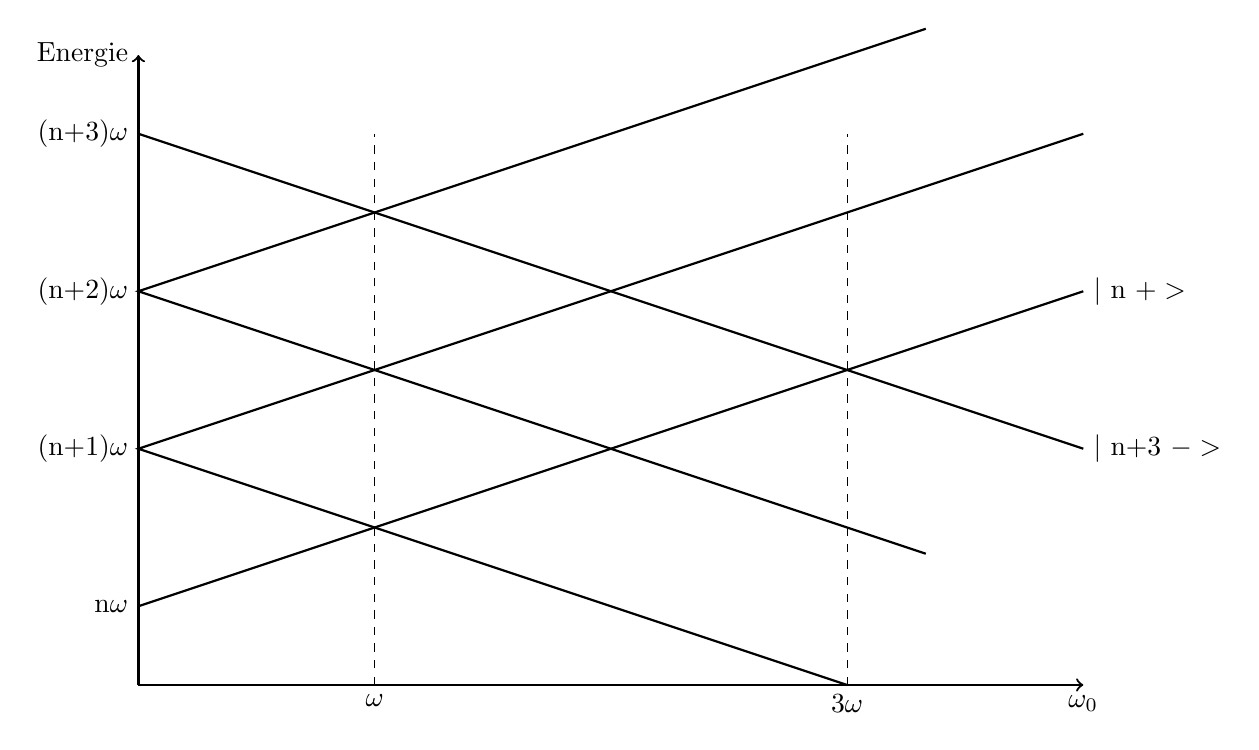
\begin{tikzpicture}
%\draw [dashed, gray] (2,5) -- (2,0) node [below, black] {};
% axes
\draw [thick, ->] (0,0) -- (0,8) node [left] {Energie};
\draw [thick, ->] (0,0) -- (12,0) node [below] {$\omega_0$};
% verticales
\draw [dashed] (3,0) node [below] {$\omega$} -- (3,7);
\draw [dashed] (9,0) node [below] {$3\omega$} -- (9,7);
% obliques y = x/3 + b
\draw [thick] (0,1) node [left] {n$\omega$} -- (12,5) node [right] {$|$ n $+>$};
\draw [thick] (9,0) -- (0,3) node [left] {(n$+1)\omega$} -- (12,7);
\draw [thick] (10,1.66666) -- (0,5) node [left] {(n$+2)\omega$} -- (10,8.33333);
\draw [thick] (12,3) node [right] {$|$ n$+3\ ->$} -- (0,7) node [left] {(n$+3)\omega$};
\end{tikzpicture} \end{center}


%%%%%%%%%%%%%%%%%%%%%%%%%%%%
